% !TeX program = xelatex
\documentclass[a4paper,10pt]{article}

% ============================================================================
% សន្លឹកកិច្ចការសិស្សបំពេញចន្លោះ ស-ខ្មៅ និងប្លង់ក្ដារខៀន/ចម្លើយគ្រូ (គ្មាន LCD / គ្មានកន្ត្រៃ)
% មេរៀនទី២ (១.១)៖ ភាពចែកដាច់នឹង 2, 5, 3, 9, 4 និង 8 — ត្រូវគ្នា ១០០% នឹង LS_Plan_DIV21.tex
% ============================================================================
\usepackage[a4paper, left=1.0cm, right=1.0cm, top=0.75cm, bottom=1.00cm, footskip=0.52cm]{geometry}
\usepackage{amsmath}
\usepackage{unicode-math}
\usepackage{fontspec}
\usepackage{array, colortbl}
\usepackage[table]{xcolor}
\usepackage{enumitem}
\usepackage{pifont}
\usepackage{fancyhdr}
\usepackage{lastpage}
\usepackage{tikz}
\usepackage[most]{tcolorbox}
\usetikzlibrary{calc, arrows.meta, decorations.pathreplacing, positioning, babel}

\makeatletter
\let\@expl@@@mark@update@singlecol@structures@@\relax
\makeatother

\providecommand{\NGSFindFonts}{%
  \IfFileExists{C:/Windows/Fonts/cambria.ttc}{%
    \def\NGSSysPath{C:/Windows/Fonts/}%
    \def\NGSUserPath{C:/Users/KIT/AppData/Local/Microsoft/Windows/Fonts/}%
  }{%
    \IfFileExists{./fonts/KhmerOSsiemreap.ttf}{\def\NGSSysPath{./fonts/}\def\NGSUserPath{./fonts/}}{%
    \IfFileExists{../fonts/KhmerOSsiemreap.ttf}{\def\NGSSysPath{../fonts/}\def\NGSUserPath{../fonts/}}{%
    \IfFileExists{../../fonts/KhmerOSsiemreap.ttf}{\def\NGSSysPath{../../fonts/}\def\NGSUserPath{../../fonts/}}{%
    \IfFileExists{../../../fonts/KhmerOSsiemreap.ttf}{\def\NGSSysPath{../../../fonts/}\def\NGSUserPath{../../../fonts/}}{%
    \IfFileExists{../../../../fonts/KhmerOSsiemreap.ttf}{\def\NGSSysPath{../../../../fonts/}\def\NGSUserPath{../../../../fonts/}}{%
    \IfFileExists{../../../../../fonts/KhmerOSsiemreap.ttf}{\def\NGSSysPath{../../../../../fonts/}\def\NGSUserPath{../../../../../fonts/}}{%
    \IfFileExists{../../../../../../fonts/KhmerOSsiemreap.ttf}{\def\NGSSysPath{../../../../../../fonts/}\def\NGSUserPath{../../../../../../fonts/}}{%
      \def\NGSSysPath{../../../../../../../fonts/}\def\NGSUserPath{../../../../../../../fonts/}%
    }}}}}}}%
  }%
}
\NGSFindFonts

\setmathfont[Path={\NGSSysPath}, FontIndex=1, Scale=1.02]{cambria.ttc}
\defaultfontfeatures{Ligatures=TeX}

\setmainfont[
  Path={\NGSUserPath}, Extension=.ttf, Script=Khmer,
  BoldFont={KhmerOSsiemreap}, BoldFeatures={FakeBold=1.8},
  ItalicFont={KhmerOSsiemreap}, ItalicFeatures={FakeSlant=0.25},
  BoldItalicFont={KhmerOSsiemreap}, BoldItalicFeatures={FakeBold=1.8, FakeSlant=0.25}
]{KhmerOSsiemreap}

\newfontfamily\muol[Path={\NGSUserPath}, Extension=.ttf, Script=Khmer]{KhmerOSmuollight}
\newfontfamily\TimesEn[Path={\NGSSysPath}, Extension=.ttf, BoldFont={timesbd}, ItalicFont={timesi}, BoldItalicFont={timesbi}]{times}
\newfontfamily\CalibriFont[Path={\NGSSysPath}, Extension=.ttf]{calibri}

\XeTeXlinebreaklocale "km"
\XeTeXlinebreakskip = 0pt plus 1pt minus 0.1pt

\definecolor{panelgray}{gray}{0.94}
\definecolor{headgray}{gray}{0.85}

\pagestyle{fancy}
\fancyhf{}
\renewcommand{\headrulewidth}{0pt}
\fancyfoot[L]{\fontsize{7.4pt}{9.5pt}\selectfont អនុវិទ្យាល័យព្រះក្រសាំង \en{|} គ្រូ៖ ហុក ប៊ុនថែន \en{|} មេរៀនទី២ (១.១) ភាពចែកដាច់នឹង \en{2, 5, 3, 9, 4, 8} \en{|} ថ្ងៃព្រហស្បតិ៍ ទី១២ ខែវិច្ឆិកា ឆ្នាំ២០២៦}
\fancyfoot[R]{\fontsize{7.8pt}{10pt}\selectfont ទំព័រ \en{\thepage\ / \pageref{LastPage}}}

\setlength{\parindent}{0pt}
\setlength{\parskip}{0pt}
\setlength{\tabcolsep}{4pt}
\newcolumntype{L}[1]{>{\raggedright\arraybackslash}p{#1}}
\newcolumntype{C}[1]{>{\centering\arraybackslash}p{#1}}

\newcommand{\en}[1]{{\TimesEn #1}}
\newcommand{\enbf}[1]{{\TimesEn\bfseries #1}}
\newcommand{\unit}[1]{\,\text{\en{#1}}}
\newcommand{\cnum}[1]{\mbox{\fontsize{10pt}{12pt}\selectfont\ding{\numexpr181+#1\relax}}}
\newcommand{\chkbox}{\tikz[baseline=-0.15ex]\draw[black, line width=0.85pt, fill=white] (0,0) rectangle (0.24cm,0.24cm);}
\newcommand{\ansbox}[1][1.75cm]{\,\tikz[baseline=-0.65ex]\draw[black, line width=0.65pt, fill=white] (0,0) rectangle (#1, 0.42cm);\,}
\newcommand{\dbox}{\,\tikz[baseline=-0.35ex]\draw[black, line width=0.75pt, fill=white] (0,0) rectangle (0.38cm,0.38cm);\,}
\newcommand{\dotline}[1][2.2cm]{\makebox[#1]{\dotfill}}

\newcommand{\pagebanner}[2]{%
  \begin{tcolorbox}[
    enhanced, sharp corners, colback=headgray, colframe=black,
    boxrule=1.05pt, boxsep=1pt, top=2.5pt, bottom=2.5pt, left=6pt, right=6pt,
    after skip=3.5pt
  ]
    {\muol\fontsize{9.0pt}{13.2pt}\selectfont #1}\hfill{\fontsize{8.0pt}{11.2pt}\selectfont\textbf{#2}}
  \end{tcolorbox}%
}

\newcommand{\secstrip}[2]{%
  \vspace{3pt}%
  \begin{tcolorbox}[
    enhanced, sharp corners, colback=panelgray, colframe=black,
    boxrule=0.8pt, boxsep=0.8pt, top=2pt, bottom=2pt, left=5pt, right=5pt,
    after skip=3pt
  ]
    {\muol\fontsize{8.5pt}{12.2pt}\selectfont #1}\hfill{\fontsize{7.8pt}{10.8pt}\selectfont\textit{#2}}
  \end{tcolorbox}%
}

\begin{document}
\fontsize{9.5pt}{14.5pt}\selectfont

% ============================================================================
% ទំព័រទី ១៖ សន្លឹកកិច្ចការសិស្ស (ផ្នែកមុខ៖ E1 -> E2 -> E3)
% ============================================================================
\pagebanner{សន្លឹកកិច្ចការសិស្ស \enbf{(}១\enbf{.}១ ភាពចែកដាច់នឹង \enbf{2, 5, 3, 9, 4, 8)} \enbf{--} ផ្នែកមុខ}{ថ្នាក់ទី៧ \en{|} សៀវភៅគោល ទំ.១៥--១៧}

\begin{tcolorbox}[
  enhanced, sharp corners, colback=white, colframe=black,
  boxrule=0.8pt, boxsep=1.5pt, top=3.5pt, bottom=3.5pt, left=5pt, right=5pt,
  after skip=4pt
]
  \fontsize{9.0pt}{13.0pt}\selectfont
  \textbf{ឈ្មោះសិស្ស៖} \dotline[4.3cm] \quad
  \textbf{សមាជិកក្រុម៖} \dotline[4.3cm] \quad
  \textbf{ថ្នាក់ទី៖} ៧\dotline[0.9cm] \quad
  \textbf{ក្រុមទី៖} \dotline[1.0cm]
\end{tcolorbox}

% --- E1 Engage ---
\secstrip{ផ្នែកទី ១ \enbf{(E1 - Engage)} ៖ បេសកកម្មអន្ទាក់លេខខាងចុងចំពោះតួចែក $3$}{រយៈពេល ៣ នាទី (គូស \ding{51} ក្នុង \chkbox)}

\begin{tcolorbox}[
  enhanced, sharp corners, colback=white, colframe=black,
  boxrule=0.8pt, boxsep=2pt, top=4pt, bottom=4pt, left=6pt, right=6pt
]
  គេពិនិត្យចំនួន $123$ និង $23$ ថាតើចែកដាច់នឹង $3$ ដែរឬទេ៖\\[2.5pt]
  $\bullet$ \chkbox\ \textbf{សិស្ស ក៖} «លេខ $123$ និង $23$ សុទ្ធតែមានលេខខាងចុងជាលេខ $3$ ដូច្នេះវាចែកដាច់នឹង $3$ ទាំងពីរ!»\\[2pt]
  $\bullet$ \chkbox\ \textbf{សិស្ស ខ៖} «$123$ ចែកដាច់នឹង $3$ ($123\div 3=41$) ប៉ុន្តែ $23$ ចែកនឹង $3$ បាន $7$ នៅសល់សំណល់ \dotline[0.9cm] មិនដាច់ទេ!»
\end{tcolorbox}

\vfill

% --- E2 Explore ---
\secstrip{ផ្នែកទី ២ \enbf{(E2 - Explore)} ៖ រុករកគ្រួសារទាំង ៣ នៃភាពចែកដាច់ (ទំ.១៥--១៧)}{រយៈពេល ១១ នាទី}

\textbf{សកម្មភាព ១ (\en{E2-A} — ៣.៥ នាទី)៖ ក. ភាពចែកដាច់នឹង $2$ និង $5$ (ទំ.១៥--១៦)}

\begin{tcolorbox}[
  enhanced, sharp corners, colback=white, colframe=black,
  boxrule=0.8pt, boxsep=2pt, top=3.5pt, bottom=3.5pt, left=6pt, right=6pt
]
  $\bullet$ $42,\ 56,\ 198,\ 210$ សុទ្ធតែចែកដាច់នឹង $2$ ព្រោះមានលេខខាងចុងជាលេខ \dotline[1.5cm] (\emph{ចំនួនគត់គូ}) ។\\[2pt]
  $\bullet$ $70,\ 95,\ 160,\ 525$ សុទ្ធតែចែកដាច់នឹង $5$ ព្រោះមានលេខខាងចុងជាលេខ \dotline[0.9cm] ឬ \dotline[0.9cm] ។\\[2.5pt]
  $\bullet$ \textbf{ប្រតិបត្តិទំ.១៦៖} បំពេញលេខក្នុងប្រអប់ $154\dbox$ ដើម្បីឱ្យចែកដាច់នឹង $2$ ផង និង $5$ ផង៖ $\dbox =$ \ansbox[1.2cm] ។
\end{tcolorbox}

\vspace{3pt}
\textbf{សកម្មភាព ២ (\en{E2-B} — ៤ នាទី)៖ ខ. ភាពចែកដាច់នឹង $3$ និង $9$ (ទំ.១៦)}

\begin{tcolorbox}[
  enhanced, sharp corners, colback=white, colframe=black,
  boxrule=0.8pt, boxsep=2pt, top=3.5pt, bottom=3.5pt, left=6pt, right=6pt
]
  $\bullet$ \textbf{ចែកដាច់នឹង $3$៖} $195 \to 1+9+5 =$ \dotline[0.9cm] $\mid$ $927 \to 9+2+7 =$ \dotline[0.9cm] $\mid$ $1\,005 \to 1+0+0+5 =$ \dotline[0.9cm] (សុទ្ធតែចែកដាច់នឹង $3$)\\[2.5pt]
  $\bullet$ \textbf{ចែកដាច់នឹង $9$៖} $216 \to 2+1+6 =$ \dotline[0.9cm] $\mid$ $828 \to 8+2+8 =$ \dotline[0.9cm] $\mid$ $2\,106 \to 2+1+0+6 =$ \dotline[0.9cm] (សុទ្ធតែចែកដាច់នឹង $9$)
\end{tcolorbox}

\vspace{3pt}
\textbf{សកម្មភាព ៣ (\en{E2-C} — ៣.៥ នាទី)៖ គ. ភាពចែកដាច់នឹង $4$ និង $8$ (ទំ.១៧)}

\begin{tcolorbox}[
  enhanced, sharp corners, colback=white, colframe=black,
  boxrule=0.8pt, boxsep=2pt, top=3.5pt, bottom=3.5pt, left=6pt, right=6pt
]
  $\bullet$ \textbf{ចែកដាច់នឹង $4$៖} $1\underline{24},\ 8\underline{32},\ 1\,0\underline{00}$ មានលេខខាងចុង \dotline[1.1cm] ខ្ទង់ ($24,\ 32,\ 00$) ចែកដាច់នឹង $4$ ។\\[2pt]
  $\bullet$ \textbf{ចែកដាច់នឹង $8$៖} $3\,\underline{128},\ 5\,\underline{048},\ 7\,\underline{120}$ មានលេខខាងចុង \dotline[1.1cm] ខ្ទង់ ($128,\ 048,\ 120$) ចែកដាច់នឹង $8$ ។
\end{tcolorbox}

\vfill

% --- E3 Explain ---
\secstrip{ផ្នែកទី ៣ \enbf{(E3 - Explain)} ៖ តារាងសង្ខេបក្បួនចែកដាច់ និងធនាគារហេតុផល \enbf{B\&W}}{រយៈពេល ៦ នាទី}

\begin{tcolorbox}[
  enhanced, sharp corners, colback=white, colframe=black,
  boxrule=0.85pt, boxsep=2pt, top=3.5pt, bottom=3.5pt, left=6pt, right=6pt
]
  ១) មួយចំនួនចែកដាច់នឹង $\mathbf{2}$ កាលណាវាជាចំនួនគត់\dotline[1.2cm]; ចែកដាច់នឹង $\mathbf{5}$ កាលណាលេខខាងចុងជា \dotline[0.8cm] ឬ \dotline[0.8cm] ។\\[2pt]
  ២) មួយចំនួនចែកដាច់នឹង $\mathbf{3}$ (ឬ $\mathbf{9}$) កាលណា \dotline[3.0cm] នៃចំនួននោះចែកដាច់នឹង $3$ (ឬ $9$) ។\\[2pt]
  ៣) មួយចំនួនចែកដាច់នឹង $\mathbf{4}$ កាលណាលេខខាងចុង\dotline[1.3cm]ខ្ទង់ $\div 4$; ចែកដាច់នឹង $\mathbf{8}$ កាលណាលេខខាងចុង\dotline[1.3cm]ខ្ទង់ $\div 8$ ។\\[3pt]
  \tikz\draw[black, dashed, line width=0.5pt] (0,0) -- (18.4cm,0);\\[3pt]
  \fontsize{8.7pt}{12.6pt}\selectfont
  \textbf{ធនាគារហេតុផល (\en{Warrant Bank})៖} \quad
  \cnum{1} ខ្ទង់រាយ ($2, 5$) \quad
  \cnum{2} ផលបូកខ្ទង់ ($3, 9$) \quad
  \cnum{3} ២ ខ្ទង់ចុង ($4$) / ៣ ខ្ទង់ចុង ($8$) \quad
  \cnum{4} ផ្ទៀងលក្ខខណ្ឌរួមគ្នាទាំងអស់
\end{tcolorbox}

% ============================================================================
% ទំព័រទី ២៖ សន្លឹកកិច្ចការសិស្ស (ផ្នែកខាងខ្នង៖ E4 -> E5 -> កិច្ចការផ្ទះ)
% ============================================================================
\clearpage
\pagebanner{សន្លឹកកិច្ចការសិស្ស \enbf{(}១\enbf{.}១ ភាពចែកដាច់នឹង \enbf{2, 5, 3, 9, 4, 8)} \enbf{--} ផ្នែកខាងខ្នង}{ថ្នាក់ទី៧ \en{|} សៀវភៅគោល ទំ.១៥--១៧, ២៤}

% --- E4 Elaborate ---
\secstrip{ផ្នែកទី ៤ \enbf{(E4 - Elaborate)} ៖ លំហាត់គំរូតាមសៀវភៅគោល ទំ.១៥, ទំ.១៦ និង ទំ.១៧}{រយៈពេល ១០ នាទី}

\begin{tcolorbox}[
  enhanced, sharp corners, colback=white, colframe=black,
  boxrule=0.8pt, boxsep=2.5pt, top=4pt, bottom=4pt, left=6pt, right=6pt
]
  $\bullet$ \textbf{១) គំរូទំ.១៥៖} គេឱ្យផលបូក $9\,018 + 1\,457$ និង $1\,995 + 1\,329$ ។ ដោយមិនធ្វើវិធីចែក ចូរប្រាប់ផលបូកដែល៖\\[2.5pt]
  \hspace*{0.3cm}ក. ចែកដាច់នឹង $2$ គឺផលបូក \dotline[3.0cm] $=$ \ansbox[1.8cm] (ព្រោះខ្ទង់រាយ $5+9=14$ ជាលេខគូ — \cnum{1})\\[2.5pt]
  \hspace*{0.3cm}ខ. ចែកដាច់នឹង $5$ គឺផលបូក \dotline[3.0cm] $=$ \ansbox[1.8cm] (ព្រោះខ្ទង់រាយ $8+7=15$ បញ្ចប់ដោយ $5$ — \cnum{1})\\[3.5pt]
  $\bullet$ \textbf{២) គំរូទំ.១៦៖} បំពេញប្រអប់ $200\dbox$ ដើម្បីឱ្យចែកដាច់នឹង $3$ ផង និង $9$ ផង៖ $2+0+0+\dbox = 9 \implies \dbox =$ \ansbox[1.2cm] (\cnum{2})\\[3.5pt]
  $\bullet$ \textbf{៣) គំរូ ១ និង ២ ទំ.១៧៖} ក. បំពេញប្រអប់ $112\,23\dbox$ ដើម្បីឱ្យចែកដាច់នឹង $4$ ផង និង $8$ ផង៖ $\dbox =$ \ansbox[1.2cm] (\cnum{3}, \cnum{4})\\[2.5pt]
  \hspace*{0.3cm}ខ. ពីឆ្នាំ $1999$ ដល់ឆ្នាំ $2010$ តើឆ្នាំណាខ្លះចែកដាច់នឹង $4$ ផង និង $8$ ផង? ចម្លើយ៖ \ansbox[3.2cm]\\[3pt]
  \fontsize{8.8pt}{12.6pt}\selectfont
  \textbf{ឆ្លុះបញ្ចាំង (\en{EIA Looking-Back})៖} បើដាក់ $\dbox = 6$ ក្នុង $112\,236$ តើ $236 \div 8$ ចែកដាច់ដែរឬទេ? ចម្លើយ៖ \dotline[2.4cm] !
\end{tcolorbox}

\vfill

% --- E5 Evaluate ---
\secstrip{ផ្នែកទី ៥ \enbf{(E5 - Evaluate)} ៖ ប្រតិបត្តិ (ទំ.១៦--១៧) សំណួរវិនិច្ឆ័យ \enbf{A--D} និងសំបុត្រចេញ}{រយៈពេល ១០ នាទី}

\begin{tcolorbox}[
  enhanced, sharp corners, colback=white, colframe=black,
  boxrule=0.8pt, boxsep=2.5pt, top=4pt, bottom=4pt, left=6pt, right=6pt
]
  \textbf{១) ប្រតិបត្តិជាក្រុមតូច ៣ នាក់ (សៀវភៅគោល ទំ.១៦ និង ទំ.១៧)៖}\\[3pt]
  $\bullet$ \textbf{ក. (ទំ.១៦)៖} គេមានចំនួនបីខ្ទង់ $7\dbox 8$ ។ បំពេញប្រអប់ដើម្បីឱ្យចែកដាច់នឹង $3$ ផង និង $9$ ផង៖ $\dbox =$ \ansbox[1.3cm] (\cnum{2})\\[3pt]
  $\bullet$ \textbf{ខ. (ទំ.១៧)៖} គេមានចំនួនប្រាំខ្ទង់ $734\dbox 0$ ។ បំពេញគ្រប់តម្លៃនៃប្រអប់ដើម្បីឱ្យចំនួននោះ៖\\[2pt]
  \hspace*{0.3cm}១) ចែកដាច់នឹង $4$៖ $\dbox \in$ \ansbox[3.4cm] \qquad ២) ចែកដាច់នឹង $8$៖ $\dbox \in$ \ansbox[2.8cm] (\cnum{3})\\[3.5pt]
  \textbf{២) បិទបេសកកម្ម \en{E1}៖} សិស្ស \dotline[1.0cm] ត្រឹមត្រូវ ព្រោះផលបូកខ្ទង់នៃ $23$ គឺ $2+3 =$ \dotline[0.9cm] មិនចែកដាច់នឹង $3$ ទេ ។
\end{tcolorbox}

\vspace{3.5pt}

\begin{tcolorbox}[
  enhanced, sharp corners, colback=white, colframe=black,
  boxrule=0.8pt, boxsep=2.5pt, top=4pt, bottom=4pt, left=6pt, right=6pt
]
  \textbf{៣) សំណួរវិនិច្ឆ័យ \en{A--D} (តើប្រយោគមួយណាត្រឹមត្រូវ? — គូសរង្វង់ រួចលើកម្រាមដៃ ១--៤)៖}\\[3pt]
  \textbf{\en{A.}} $4\,136$ ចែកដាច់នឹង $9$ \quad
  \textbf{\en{B.}} $5\,040$ ចែកដាច់នឹង $2, 5, 9$ និង $8$ \quad
  \textbf{\en{C.}} $1\,234$ ចែកដាច់នឹង $4$ \quad
  \textbf{\en{D.}} $2\,133$ ចែកដាច់នឹង $2$ និង $3$\\[4pt]
  \tikz\draw[black, dashed, line width=0.5pt] (0,0) -- (18.4cm,0);\\[3.5pt]
  \textbf{៤) សំបុត្រចេញ ៦០ វិនាទី៖} បំពេញលេខក្នុងប្រអប់ $4\,2\dbox 0$ ដើម្បីឱ្យចែកដាច់នឹង $9$៖ $4+2+\dbox+0=9 \implies \dbox =$ \ansbox[1.4cm] ។
\end{tcolorbox}

\vfill

% --- Homework ---
\begin{tcolorbox}[
  enhanced, sharp corners, colback=panelgray, colframe=black,
  boxrule=0.95pt, boxsep=2.5pt, top=4pt, bottom=4pt, left=6pt, right=6pt
]
  {\muol\fontsize{9.0pt}{13.0pt}\selectfont កិច្ចការផ្ទះ \enbf{(}សៀវភៅគោល ទំ.២៤ លេខ ២ និងលំហាត់ពង្រឹង\enbf{)}}\\[3pt]
  \fontsize{8.8pt}{12.8pt}\selectfont
  $\bullet$ \textbf{លេខ ២ (ទំ.២៤)៖} គេមានចំនួនប្រាំខ្ទង់ $734\dbox 0$ ។ បំពេញលេខក្នុងប្រអប់ដើម្បីឱ្យចំនួននោះចែកដាច់៖ ក. នឹង $2$ ផង និង $5$ ផង \quad ខ. នឹង $3$ ផង និង $9$ ផង ។\\[2pt]
  $\bullet$ \textbf{លំហាត់ពង្រឹង៖} ក្នុងចំណោមចំនួន $6\,480;\ 3\,125;\ 7\,314;\ 9\,108$ តើចំនួនណាខ្លះចែកដាច់នឹង៖ (១) $2$ និង $5$? \quad (២) $3$ និង $9$? \quad (៣) $4$ និង $8$?
\end{tcolorbox}

% ============================================================================
% ទំព័រទី ៣៖ ទំព័រគ្រូបង្រៀន (គំរូប្លង់ក្ដារខៀន ៣ ផ្នែក + ចម្លើយផ្ទៀងផ្ទាត់រហ័ស)
% ============================================================================
\clearpage
\pagebanner{ទំព័រគ្រូបង្រៀន ៖ ប្លង់ក្ដារខៀន \enbf{(}គ្មាន \enbf{LCD)} និងចម្លើយផ្ទៀងផ្ទាត់រហ័ស}{១.១ ភាពចែកដាច់នឹង \en{2, 5, 3, 9, 4, 8} (\en{DIV21})}

\secstrip{១. គំរូប្លង់បែងចែកក្ដារខៀន ៣ ផ្នែក សម្រាប់ថ្នាក់រៀនគ្មាន \enbf{LCD}}{សម្រាប់គ្រូប្រើដីស/ហ្វឺត}

\begin{center}
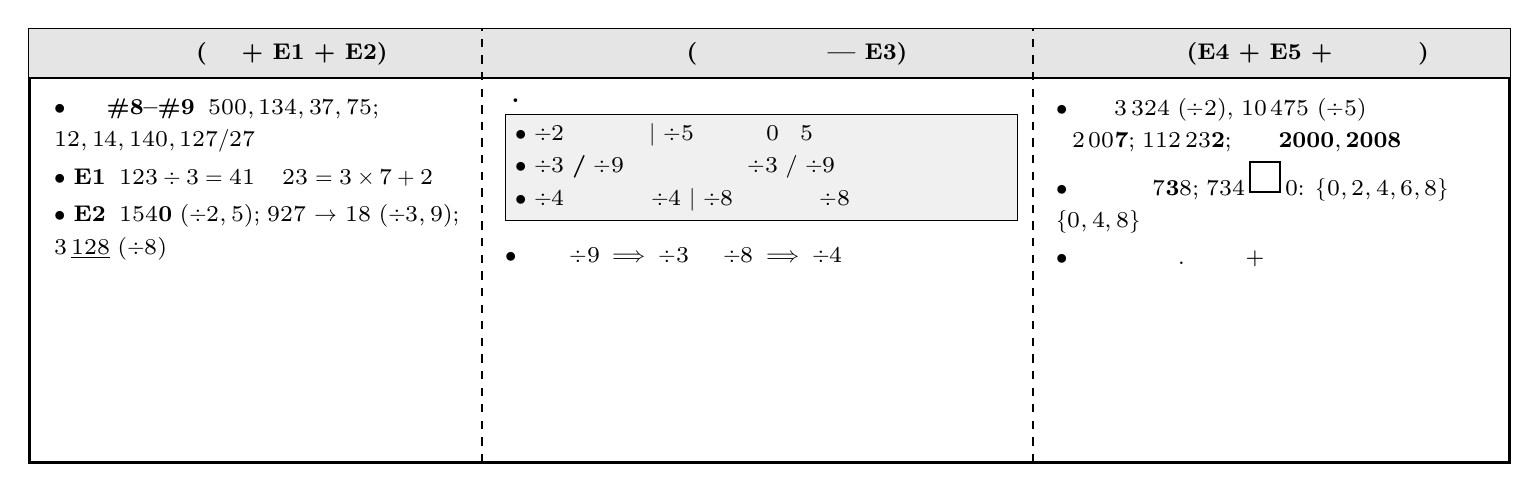
\begin{tikzpicture}[x=1cm, y=1cm, every node/.style={font=\fontsize{8.2pt}{11.6pt}\selectfont, text=black}]
  \draw[black, line width=1.1pt] (0,0) rectangle (18.8,5.50);
  \fill[gray!20] (0,4.88) rectangle (18.8,5.50);
  \draw[black, line width=0.7pt] (0,4.88) -- (18.8,4.88);
  \draw[black, dashed, line width=0.7pt] (5.75,0) -- (5.75,5.50);
  \draw[black, dashed, line width=0.7pt] (12.75,0) -- (12.75,5.50);

  \node at (2.875,5.19) {\textbf{ផ្នែកឆ្វេង (កំណែ + \en{E1} + \en{E2})}};
  \node at (9.25,5.19) {\textbf{ផ្នែកកណ្ដាល (ខ្លឹមសារគោលរក្សាទុក — \en{E3})}};
  \node at (15.775,5.19) {\textbf{ផ្នែកស្ដាំ (\en{E4} + \en{E5} + កិច្ចការផ្ទះ)}};

  % Left
  \node[anchor=north west, text width=5.30cm] at (0.20,4.74) {%
    $\bullet$ \textbf{កំណែ \#8–\#9៖} $500, 134, 37, 75$; $12, 14, 140, 127/27$\\[2pt]
    $\bullet$ \textbf{\en{E1}៖} $123\div 3=41$ តែ $23 = 3\times 7 + 2$\\[2pt]
    $\bullet$ \textbf{\en{E2}៖} $154\mathbf{0}$ ($\div 2,5$); $927\to 18$ ($\div 3,9$); $3\,\underline{128}$ ($\div 8$)
  };

  % Center
  \node[anchor=north west, text width=6.65cm] at (5.92,4.74) {%
    {\muol\fontsize{8.3pt}{11.8pt}\selectfont ១\enbf{.}១ ភាពចែកដាច់នៃចំនួនគត់}\\[3pt]
    \tikz\node[draw=black, fill=gray!12, inner sep=3.5pt, text width=6.25cm]{%
      $\bullet$ \textbf{$\div 2$៖} ខ្ទង់រាយគូ $\mid$ \textbf{$\div 5$៖} ខ្ទង់រាយ $0$ ឬ $5$\\
      $\bullet$ \textbf{$\div 3$ / $\div 9$៖} ផលបូកលេខតាមខ្ទង់ $\div 3$ / $\div 9$\\
      $\bullet$ \textbf{$\div 4$៖} ២ ខ្ទង់ចុង $\div 4$ $\mid$ \textbf{$\div 8$៖} ៣ ខ្ទង់ចុង $\div 8$
    };\\[3.5pt]
    $\bullet$ ចំណាំ៖ $\div 9 \implies \div 3$ និង $\div 8 \implies \div 4$
  };

  % Right
  \node[anchor=north west, text width=5.65cm] at (12.92,4.74) {%
    $\bullet$ \textbf{គំរូ៖} $3\,324$ ($\div 2$), $10\,475$ ($\div 5$)\\
    \hspace*{0.2cm}$2\,00\mathbf{7}$; $112\,23\mathbf{2}$; ឆ្នាំ $\mathbf{2000, 2008}$\\[2pt]
    $\bullet$ \textbf{ប្រតិបត្តិ៖} $7\mathbf{3}8$; $734\dbox 0$: $\{0,2,4,6,8\}$ និង $\{0,4,8\}$\\[2pt]
    $\bullet$ \textbf{កិច្ចការផ្ទះ៖} ទំ.២៤ លេខ ២ + ពង្រឹង
  };
\end{tikzpicture}
\end{center}

\vfill
\secstrip{២. ចម្លើយផ្ទៀងផ្ទាត់រហ័សសម្រាប់សន្លឹកកិច្ចការសិស្ស \enbf{(}ទំព័រ ១ និង ទំព័រ ២\enbf{)}}{\en{Answer Key}}

\begin{tcolorbox}[
  enhanced, sharp corners, colback=white, colframe=black,
  boxrule=0.8pt, boxsep=2.5pt, top=4pt, bottom=4pt, left=6pt, right=6pt
]
  \fontsize{8.8pt}{13.0pt}\selectfont
  $\bullet$ \textbf{ផ្នែក \en{E1}៖} \textbf{សិស្ស ខ} ត្រឹមត្រូវ ($23\div 3 = 7$ សល់សំណល់ $\mathbf{2}$) ។ \textbf{ផ្នែក \en{E2}៖} \en{E2-A}: លេខគូ ($0,2,4,6,8$); $0$ ឬ $5$; $\dbox = \mathbf{0}$ ។ \en{E2-B}: $15, 18, 6$ និង $9, 18, 9$ ។ \en{E2-C}: ពីរខ្ទង់ និង បីខ្ទង់ ។\\[2pt]
  $\bullet$ \textbf{ផ្នែក \en{E4}៖} ១) ក. $1\,995+1\,329 = \mathbf{3\,324}$ ($\div 2$); ខ. $9\,018+1\,457 = \mathbf{10\,475}$ ($\div 5$) ។ ២) $\dbox = \mathbf{7}$ ។ ៣) ក. $\dbox = \mathbf{2}$; ខ. ឆ្នាំ $\mathbf{2000}$ និង $\mathbf{2008}$ ។ \en{EIA}៖ មិនដាច់ទេ ($236 = 8\times 29 + 4$) ។\\[2pt]
  $\bullet$ \textbf{ផ្នែក \en{E5}៖} ១) ក. $\dbox = \mathbf{3}$ ($738$); ខ. $\div 4 \implies \mathbf{\{0,2,4,6,8\}}$, $\div 8 \implies \mathbf{\{0,4,8\}}$ ($400, 440, 480$) ។ ២) សិស្ស ខ ($5$) ។ ៣) \textbf{ជម្រើស \en{B}} ។ ៤) សំបុត្រចេញ៖ $\dbox = \mathbf{3}$ ។
\end{tcolorbox}

\vfill
\secstrip{៣. ចម្លើយលម្អិតនៃកិច្ចការផ្ទះ \enbf{(}សៀវភៅគោល ទំ.២៤ លេខ ២ និងលំហាត់ពង្រឹង\enbf{)}}{សៀវភៅគោល ទំ.២៤}

\begin{tcolorbox}[
  enhanced, sharp corners, colback=white, colframe=black,
  boxrule=0.8pt, boxsep=2.5pt, top=4pt, bottom=4pt, left=6pt, right=6pt
]
  \fontsize{8.7pt}{12.8pt}\selectfont
  $\bullet$ \textbf{លេខ ២ (ទំ.២៤ — $734\dbox 0$)៖} ក. ដោយខ្ទង់រាយជាលេខ $0$ ស្រាប់ ចំនួននេះចែកដាច់នឹង $2$ ផង និង $5$ ផងចំពោះ\textbf{គ្រប់លេខ} $\dbox \in \mathbf{\{0,1,2,3,4,5,6,7,8,9\}}$! ខ. ចែកដាច់នឹង $3$ ផង និង $9$ ផង៖ $7+3+4+\dbox+0 = 14+\dbox = 18 \implies \dbox = \mathbf{4}$ ($73\,440$) ។\\[2pt]
  $\bullet$ \textbf{លំហាត់ពង្រឹង៖} (១) $\div 2$ និង $\div 5$៖ $\mathbf{6\,480}$ ។ (២) $\div 3$ និង $\div 9$៖ $\mathbf{6\,480}$ ($18$) និង $\mathbf{9\,108}$ ($18$) [ចំណាំ៖ $7\,314 \to 15$ ចែកដាច់តែនឹង $3$ ទេ] ។ (៣) $\div 4$ និង $\div 8$៖ $\mathbf{6\,480}$ ($480\div 8=60$) [ចំណាំ៖ $9\,108$ ចែកដាច់តែនឹង $4$ ទេ ព្រោះ $108\div 8$ សល់ $4$] ។
\end{tcolorbox}

\vfill
\secstrip{៤. ចំណុចប្រុងប្រយ័ត្នគរុកោសល្យ និងកំហុសបោះពុម្ពសៀវភៅគោលសម្រាប់គ្រូ}{\en{Pedagogical \& Textbook Watchlist}}

\begin{tcolorbox}[
  enhanced, sharp corners, colback=panelgray, colframe=black,
  boxrule=0.85pt, boxsep=2.5pt, top=4pt, bottom=4pt, left=6pt, right=6pt
]
  \fontsize{8.6pt}{12.6pt}\selectfont
  $\bullet$ \textbf{កំហុសបោះពុម្ពទំ.១៥ (លំហាត់គំរូ)៖} សៀវភៅពុម្ពសរសេរចម្លើយឆ្លាស់លំដាប់ ក/ខ ហើយបោះពុម្ពខុសជា «$9018+1457 = 91575$» — តម្លៃពិតគឺ $\mathbf{10\,475}$ (ហើយតាមពិតសិស្សគ្រាន់តែបូកខ្ទង់រាយ $8+7=15$ ក៏ដឹងថាចែកដាច់នឹង $5$ ភ្លាម!) ។\\[2pt]
  $\bullet$ \textbf{ចំណាំទំ.១៧ (លំហាត់គំរូ ២)៖} ចន្លោះពីឆ្នាំ $1999$ ដល់ឆ្នាំ $2010$ សៀវភៅពុម្ពដាក់តែចម្លើយ «$2008$» ប៉ុន្តែឆ្នាំ $\mathbf{2000}$ ក៏ចែកដាច់នឹង $4$ ($2000\div 4=500$) និង $8$ ($2000\div 8=250$) ដែរ ដូច្នេះគ្រូគួរទទួលស្គាល់និងសរសើរសិស្សដែលរកឃើញទាំង $2000$ និង $2008$ ។
\end{tcolorbox}

\end{document}
